\documentclass{beamer}
\usepackage[utf8]{inputenc}
\usepackage{amssymb,amsmath,amsthm,mathtools,booktabs}

\usepackage{tikz}
\usetikzlibrary{calc} 

\newcommand{\tr}{{\text{tr}}}
\newcommand{\B}[1]{\textbf{#1}}
\newcommand{\T}[1]{\texttt{#1}}

\title{A ququart SIC for ion trap quantum computers}
\author{Matthew B. Weiss}
\institute{UMB: QBism Group}
\date{9/12/25}

\begin{document}

\frame{\titlepage}


\begin{frame}
\frametitle{Symmetric informationally complete sets}
\begin{center}
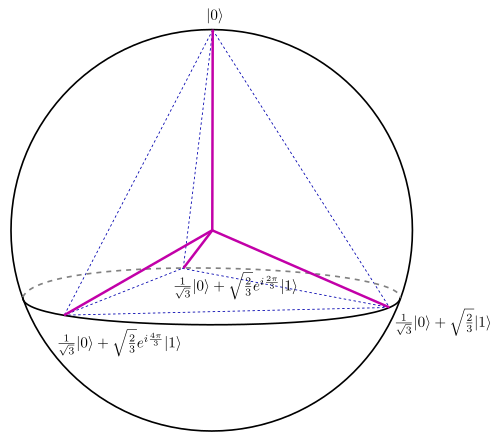
\includegraphics[scale=0.25]{img/qubit_sic}	
\end{center}
Fix a Hilbert space $\mathcal{H}_d$. If you can find a set of $d^2$ rank-1 projectors $\{\Pi_i\}$ satisfying
\begin{align}
	\tr(\Pi_{i}\Pi_{j})=\frac{d\delta_{i,j}+1}{d+1},
\end{align}
then you've found  regular simplex inscribed in quantum state-space: a SIC!
\end{frame}

\begin{frame}
\frametitle{SIC's}
\begin{itemize}
\item SIC states (with a group covariance) have \emph{maximal magic}.
\item The corresponding POVM $\{E_i = \frac{1}{d}\Pi_i\}$ is \emph{optimal for linear quantum state tomography}.
\item A SIC-based generalization of the double-split experiment demonstrates  the \emph{inherent contextuality} of quantum theory.
\item The numbers involved in constructing a SIC have \emph{deep algebraic number theoretic significance}. 
\item The question of whether SIC's exist in all dimensions directly relates to Hilbert's 12 problem about abelian extensions of the rationals!
\end{itemize}
\end{frame}


\begin{frame}
\frametitle{The Weyl-Heisenberg Group}
Fixing $\mathcal{H}_d$, let $\omega = e^{2\pi i /d}$, and define clock and shift operators,
\begin{align}
Z|m\rangle = \omega^{m}|m\rangle && 	X|m\rangle = |m+1\rangle && X=F^\dagger Z F,
\end{align}	
where $F$ is the DFT, as well as Weyl-Heisenberg displacement operators,
\begin{align}
D_{a,b} = X^a Z^b	.
\end{align}
Save one sporadic case, the orbit of a special ``fiducial'' state $\Pi$ under the WH group gives the $d^2$ SIC states,
\begin{align}
	\Pi_{a,b}=D_{a,b} \Pi D_{a,b}^\dagger.
\end{align}
WH group covariance means:
\begin{itemize}
\item We can find fiducials more easily classically.
\item We can implement SICs more easily quantum mechanically.
\end{itemize}
\end{frame}

\begin{frame}
\frametitle{Historical flavor}
From \emph{Bell System Technical Journal}:
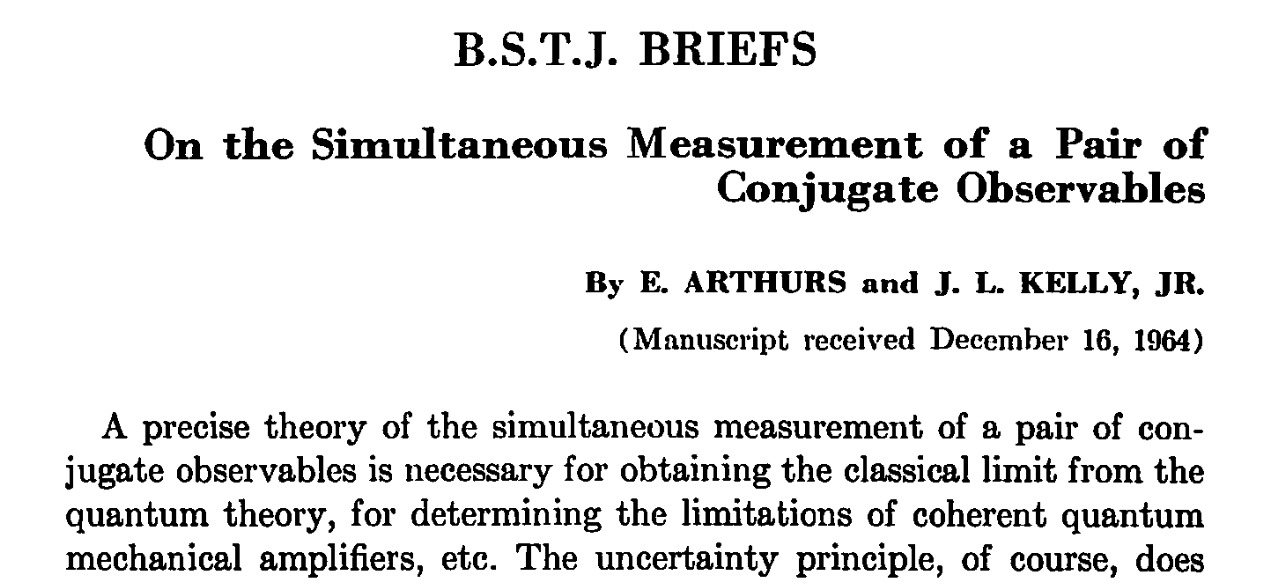
\includegraphics[scale=0.5]{img/ak_ref}	
\end{frame}

\begin{frame}
\frametitle{Arthurs-Kelly procedure}
\begin{itemize}
\item Prepare two ancillas in a special starting state.
\item Coherently shift ancilla 1 conditional on the position of the system.
\item Coherently shift ancilla 2 conditional on the momentum of the system.
\item Measure the ancillas.
\end{itemize}
 Realizes a ``Weyl-Heisenberg covariant POVM'' on the system.

\begin{itemize}
\item E.g., a coherent state measurement, or ``heterodyne'' measurement in optics.
\item Can be adapted to qudits: in particular, for a SIC measurement.
\end{itemize}
	
\end{frame}




\begin{frame}
\frametitle{Qudit Arthurs-Kelly}
Let $|\cdot \rangle$ denote discrete position states and $|\cdot\rangle_p$ denote discrete momentum states.
\begin{align}
U_{AK} &= \left(\sum_m I \otimes X^{-m} \otimes |m\rangle_p\langle m|_p	\right)\left(\sum_k X^{-k} \otimes I \otimes |k\rangle\langle k|\right),
\end{align}
where $|m\rangle_p = F|m\rangle$.
\end{frame}

\begin{frame}
\frametitle{Qudit Arthurs-Kelly}
\begin{itemize}
 \item To prepare the staring state of the two ancillas,
\begin{align}
U_{PA} &= 	\left(\sum_j |j\rangle\langle j|\otimes Z^j	\otimes I\right)\Big(I \otimes F^\dagger \otimes I\Big).
\end{align}
\item Let $|\phi\rangle$ be a SIC fiducial, and $|\psi\rangle$  the system state, then
\begin{align}
|\text{post-interaction}\rangle=U_{AK}U_{PA}\Big(|\phi^*\rangle	\otimes |\phi\rangle \otimes |\psi\rangle\Big).
\end{align}
\item 	Measuring the two ancillas gives $d^2$ possible outcomes with \begin{align}
 	P(a,b)=\frac{1}{d}\tr(\Pi_{a,b}\rho).
 \end{align}
\item Afterwards, the system is projected into the SIC state $\Pi_{a,b}$.
\end{itemize}
\end{frame}

\begin{frame}
	\frametitle{A simplification}
\begin{itemize}
\item Let  $|\psi\rangle$ an arbitrary state, and $|\phi\rangle$ be the fiducial.
\begin{align}
&\Big(\langle a| \otimes \langle b|\Big)(I\otimes F^\dagger)\left(\sum_j X^{-j}\otimes |j\rangle\langle j|\right)\Big(|\psi\rangle \otimes |\phi^*\rangle	\Big)\nonumber\\
&=\frac{1}{\sqrt{d}}\langle \phi |D_{a,b}^\dagger |\psi\rangle
\end{align}
\item The probabilities for a computational basis measurement are precisely the SIC probabilities.
\item  Just one ancilla!
\item  But afterwards, the state is projected into a computational basis state.
\end{itemize}
\end{frame}


\begin{frame}
\frametitle{A $d=4$ fiducial}
Exploit the ``monomial representation'' to write
\begin{align}
\label{fiducial}
&|\phi\rangle = \nonumber\\
&	(H \otimes I)\begin{pmatrix}1 & 0 & 0 & 0\\ 0 & e^{i\pi(-1/4)} & 0 & 0 \\ 0 & 0 & e^{i\pi (1/4)} & 0 \\ 0 & 0 & 0 & e^{i\pi (1/2)}\end{pmatrix}\frac{1}{\sqrt{5+\sqrt{5}}}\begin{pmatrix} \sqrt{2+\sqrt{5}} \\ 1 \\ 1 \\ 1 \end{pmatrix},
\end{align}	
where $H$ is the qubit Hadamard gate. 	
\end{frame}

\begin{frame}
\frametitle{Ion traps}
\begin{itemize}
\item \emph{Experimental single-setting quantum state tomography}: you implement a qubit SIC using a native quqart.
\item Can we realize a ququart SIC using two (or three) native ququarts? 
\item \emph{A universal qudit quantum processor with trapped ions}: working with $d=10$ qudits, you show how to implement a controlled exchange gate $C_{\text{EX}}$ from which one can implement $C_{\text{SUM}}$, that is, calling the controlled shift.
\item How hard is it to do the discrete Fourier transform?
\item Compare performance to tensor products of qubit SIC's in estimating observables, etc.
\end{itemize}
	
\end{frame}

\begin{frame}
\frametitle{From tomography to the Born rule}
\begin{itemize}
\item Reconstructing density matrices from SIC probabilities:
\begin{align}
\rho = \sum_i \left[(d+1)P(R_i)- \frac{1}{d}\right]\Pi_i	,
\end{align}
where $P(R_i)=\frac{1}{d}\tr(\Pi_i\rho)$.
\item Leads to an elegant reformulation of the Born rule as a consistency rule for probability assignments...
\end{itemize}
\end{frame}


\begin{frame}
\frametitle{The Born Rule}
\vspace{-2em}
\begin{center}
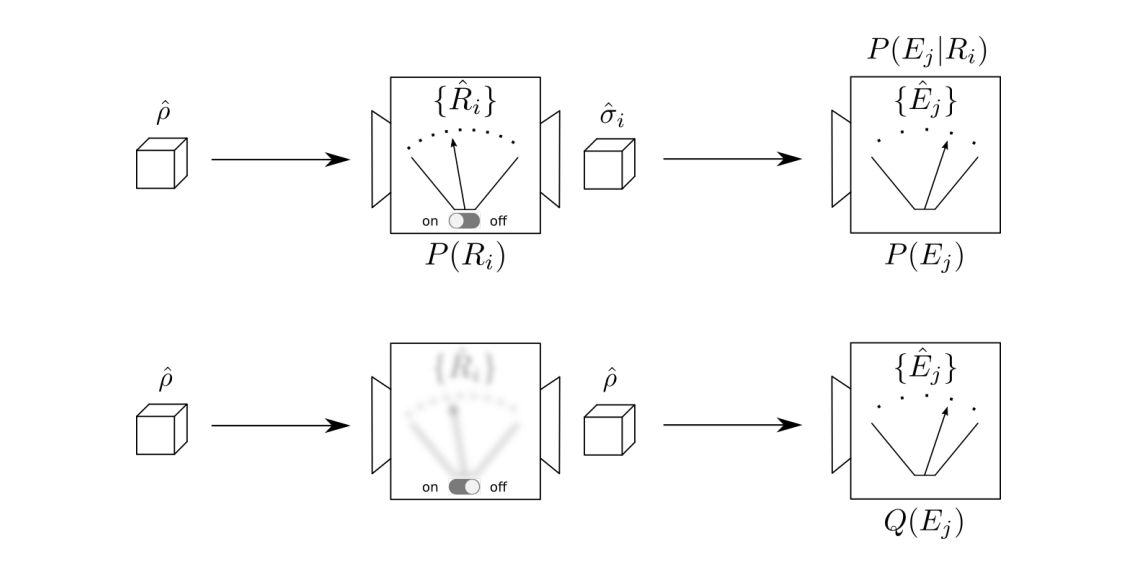
\includegraphics[scale=0.45]{img/sky_ground}	
\end{center}
\vspace{-2em}
\begin{small}
\begin{align}
P(E_j) &= \sum_i P(E_j|R_i)P(R_i)\\
Q(E_j) &= \sum_{ik} P(E_j|R_i)\Phi_{ik}P(R_k)
\end{align}
where $\Phi = P(R|R)^{-1}$ for any IC $\{R_i\}$ and $\{\sigma_i\}$.\end{small}
\end{frame}

\begin{frame}
\frametitle{The Born Rule}
\begin{itemize}
\item In particular, for a SIC:
\begin{align}
Q(E_j) &=\sum_{i} P(E_j|R_i)\left[(d+1)P(R_i)-\frac{1}{d}\right]	.
\end{align}	
\item Among all IC-POVMs with $d^2$ elements, $\lVert I - \Phi \rVert$ achieves its minimum only for SIC's.
\item Other measurements artificially exaggerate the difference between classical and quantum!
\item  Let $W(E_j)=(d+1)P(R_i)-\frac{1}{d}$: these are quasiprobabilities. 
\item Their negativity diagnoses contextuality. 
\item The more noise, the less negativity.
\end{itemize}
	
\end{frame}

\begin{frame}
\frametitle{Consistency}
Let us consider the following set of experiments:
\begin{enumerate}
\item Prepare the SIC states in turn, and then a SIC measurement. Yields matrix of probabilities $P_{ij}=P(R_i|R_j)$.
\item Prepare the computational basis states $\{\Pi_i=|i\rangle\langle i|\}$, and then performing a SIC. Yields probabilities $p_{ij} = P(R_j|\Pi_i)$.
\item Prepare the SIC states, and a computational basis measurement: $C_{ij}=P(\Pi_i|R_j)$.
\item Prepare the computational basis states, and then a computational basis measurement: $q_{ij}=P(\Pi_i|\Pi_j)$.
\end{enumerate}
	Letting $\Phi=P^{-1}$, the Born rule then demands the following consistency criterion,
\begin{align}
q = C\Phi p.	
\end{align}
Can we achieve this in the presence of noise?
\end{frame}


\begin{frame}
\frametitle{For reference, a qubit implementation}
	Let $\T{R}(k) = \begin{pmatrix}1 & 0 \\ 0 & e^{2\pi i/2^k} \end{pmatrix}$.
	\begin{align}
\T{Z}= \bigotimes_{j=0}^{n-1} \T{R}(j+1) && \T{X}=\T{F}^\dagger \T{Z}\T{F}.
\end{align}
Qudit Fourier transform:
\begin{center}
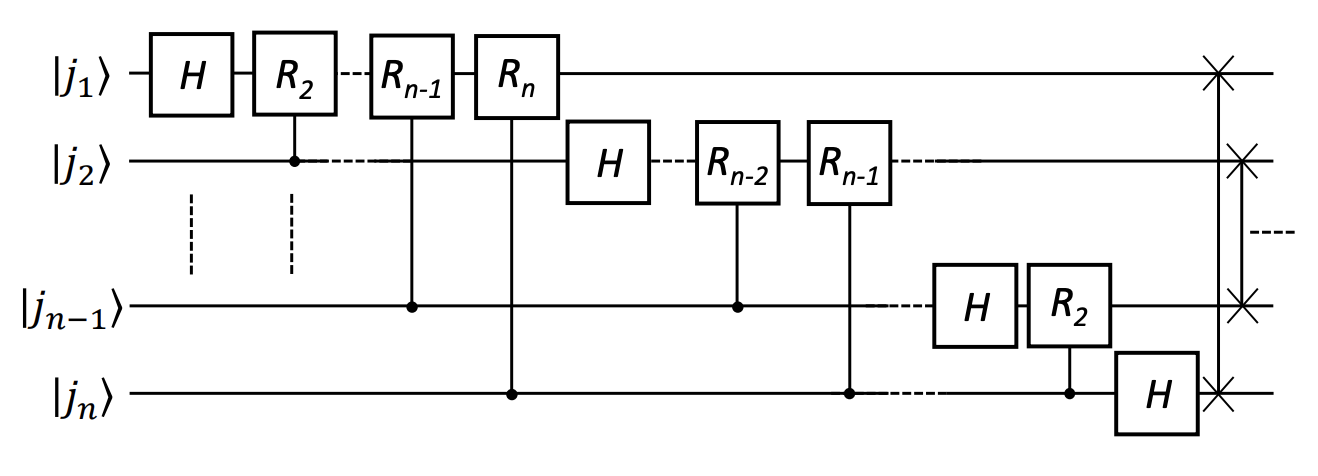
\includegraphics[scale=0.45]{img/qft.png}
\end{center}
\end{frame}

\begin{frame}
\frametitle{\T{CZ} \& \T{CX}}
\T{CZ} can be built out of a series of qudit-controlled \T{Z}'s, and \T{CX} obtained by Fourier transforming. Below: first three qubits target, second three qubits control:
\begin{center}
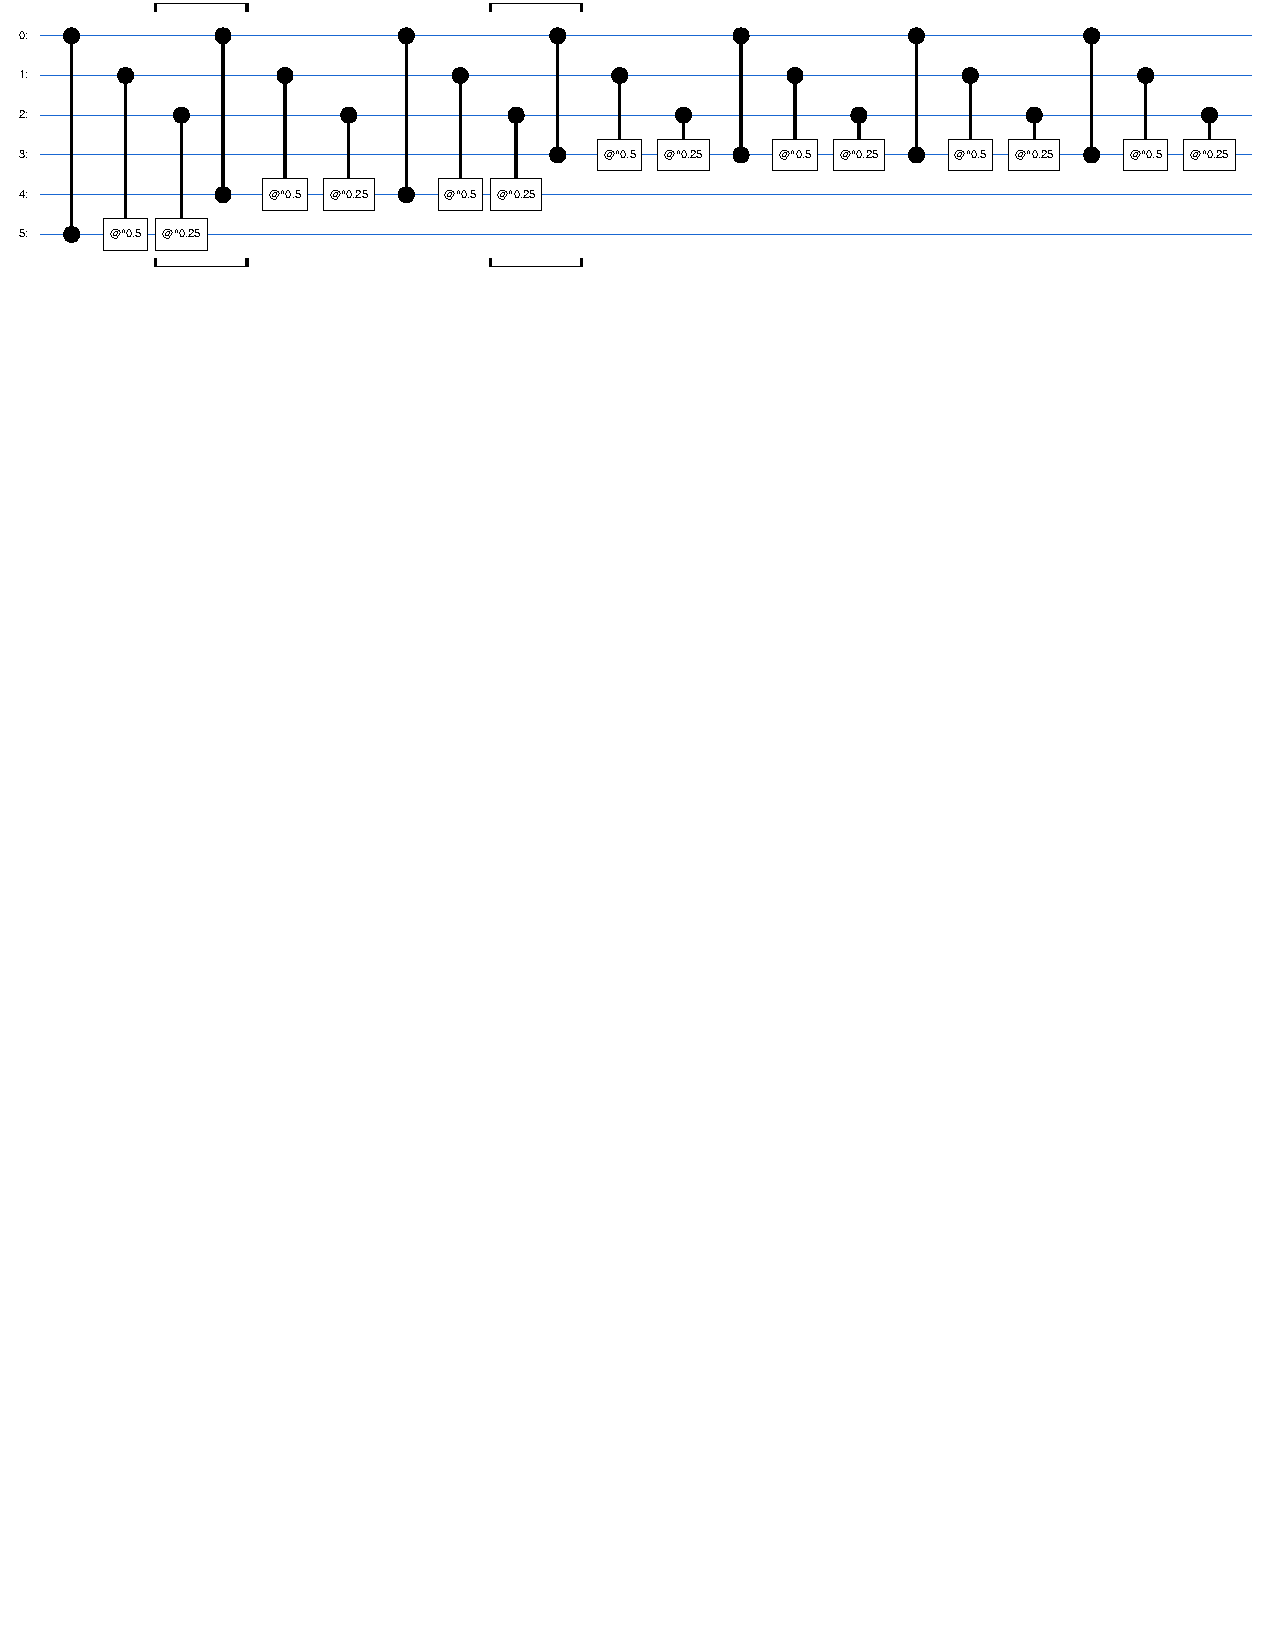
\includegraphics[scale=0.5]{img/controlled_clock.pdf}
\end{center}	
\begin{align*}
&\Big(I\otimes|0\rangle\langle0|\otimes I\otimes I + Z^4\otimes |1\rangle\langle 1| \otimes I \otimes I\Big)\\
&\Big(I\otimes I\otimes |0\rangle\langle 0| \otimes I+Z^2\otimes I\otimes |1\rangle\langle 1| \otimes I\Big)\\
&\Big(I\otimes I\otimes I\otimes |0\rangle\langle 0|+Z\otimes I\otimes I\otimes |1\rangle\langle 1|\Big)	\\
&=\sum_{m=0}^{7}Z^m \otimes |m\rangle\langle m| 
\end{align*}

\end{frame}

\begin{frame}
\frametitle{Preparing a $d=4$ fiducial}
As a circuit:
\begin{center}
 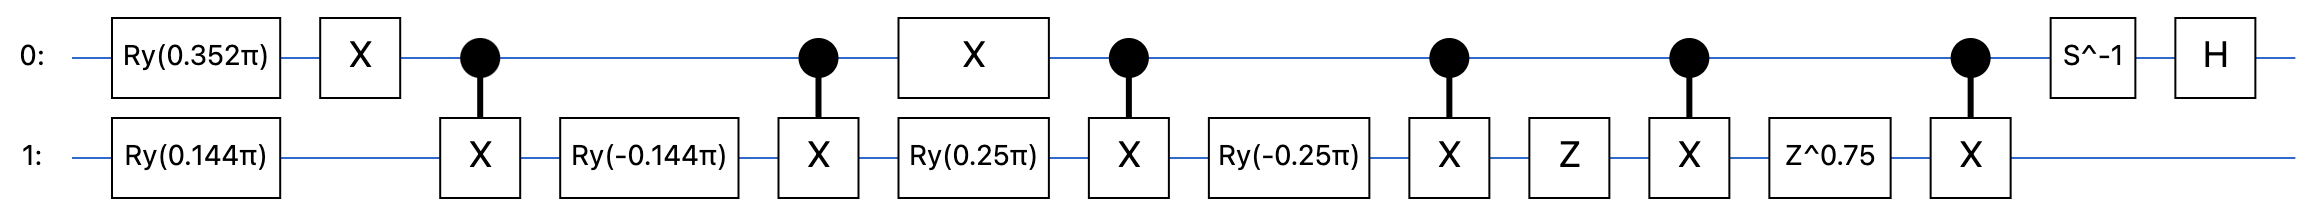
\includegraphics[scale=0.28]{img/fiducial_prep}
\end{center}   
   \end{frame}


\end{document}
